\section{Version Control with Git} 

  Git is a pretty complex version control tool. It allows you to perform different actions. We'll go over them, starting with the most basic to the most complex. In order to learn this, we should know the structure of the git history. 

\subsection{Local Git Repository} 

  When you do \texttt{git init} in a repository, you are essentially saying that you want to keep track of the history of this repository. This can obviously be done with an undo tree, which comes out-of-box in almost all text editors, but it is much more powerful. 

  \begin{definition}[Local Git Tree]
    The history of our repository is essentially a tree, with each node representing some edits composed of 
    \begin{enumerate}
      \item adding a new file 
      \item modifying a file 
      \item deleting a file
    \end{enumerate} 
    Each node is represented by a hash generated from its previous node and the corresponding edits. You can see your history using  
    \begin{lstlisting}
      git log 
    \end{lstlisting} 
    \texttt{HEAD} is a pointer to the node that reflects the state of your current repository (minus your uncommitted edits), which is usually the most recent node. 
  \end{definition} 

  Unlike most undo trees, these nodes are not added automatically. You must add them manually through a 2-step process. 

  \begin{definition}[Stage]
    You want to take a set of edits and \textbf{stage} them. This essentially tells git that these staged files/lines are going to be a part of the next node. 
  \end{definition}

  \begin{definition}[Commit]
    Then you commit your changes, which does the following. 
    \begin{enumerate}
      \item This takes all of your staged changes and packages them in a node $A$. 
      \item It looks at \texttt{HEAD}, uses \texttt{HEAD}'s hash to generate the hash of $A$, and appends $A$ to \texttt{HEAD} by having $A$ point to \texttt{HEAD}.\footnote{So nodes actually point to \textit{previous nodes}.}
      \item It moves \texttt{HEAD} to $A$. 
    \end{enumerate}
  \end{definition} 

  Therefore, when you make your first commit, you are creating a genesis node from which every other edit will be based off of. Your \texttt{HEAD} then points to this commit. This is great start, and let's add more functionality. 

  \begin{definition}[Checkout a Commit]
    You can move \texttt{HEAD} to point to a specific commit by using 
    \begin{lstlisting}
      git checkout <commit-hash>  # point to this commit  
      git checkout HEAD~N         # point to the commit $N$ nodes before HEAD
    \end{lstlisting} 
    This leaves you in a \texttt{detached head state}, which means that your head is not pointing to the end node. This is useful if you want to 
    \begin{enumerate}
      \item \textit{explore the codebase at a commit's snapshot in time}. 
    \end{enumerate}
  \end{definition} 

  Note that so far, we have described git as a linked list plus some extra head pointer. Adding to this linked list is easy since we are simply adding new edits, but deleting can be very tricky. We will first introduce how to delete the most recent $K$ commits, which is the easiest way to delete. 

  \begin{definition}[Reset] 
    Say that your history is 
    \begin{equation}
      (A) \leftarrow (B) \leftarrow (C) \leftarrow (H \mapsto D)
    \end{equation}  
    If we want to throw away commits $C$ and $D$, we can \textbf{reset} to $B$, which deletes $C, D$ and has $H$ point to $B$, giving us 
    \begin{equation}
      (A) \leftarrow (H \mapsto B)
    \end{equation} 
    \begin{enumerate}
      \item A \textbf{soft reset} means that the edits introduced in $C$ and $D$ will still be kept as unstaged changes, and so you may use them as a starting point to make your next commit. 
      \item A \textbf{hard reset} means that the edits are also completely deleted. 
    \end{enumerate}
  \end{definition} 

  Most beginners in git really know these commands when working with their history, but this is really just a glorified stack. The additional operations can be daunting because they have the risk of introducing \textit{conflicts}. 

\subsection{Conflicts} 

  \begin{definition}[Conflicts]
    A \textbf{conflict} arises when two commits contain edits that change some location independently at the same time. They occur most frequently when working with multiple branches, but they can happen even when working on a single branch. Git will tell you when there is conflict between commits $C$ and $C^\prime$ at a certain location. At this point, you will have to manually go to that location and compare the changes introduced in $C$ and $C^\prime$, called \textbf{hunks}. The conflict looks generally like this. 
    \begin{lstlisting}
      ... some code above 
      <<<<< (C)   # hunk 1
      ========
      >>>>> (C')  # hunk 2
      ... some code below
    \end{lstlisting} 

    In order to fix this conflict, you can  
    \begin{enumerate}
      \item select hunk 1 (and ignore hunk 2)
      \item select hunk 2 
      \item select both hunks (i.e. incorporate both edits) 
      \item manually delete the \texttt{>>>}, \texttt{===}, \texttt{<<<} and directly edit the file to make a custom change that overrides both hunks. 
    \end{enumerate} 
  \end{definition} 

  Choosing the option to fix a conflict may sometimes be complicated, since you may not always want to select the hunk reflected in your most recent changes, because doing that might introduce another conflict in a later commit that actually modified the old code into the new code. 

  \begin{definition}[Revert Commit] 
    Say that you have history
    \begin{equation}
      (C_1) \leftarrow (C_2) \leftarrow (C_3) \leftarrow (H \mapsto C_4)
    \end{equation} 
    You can choose to \textbf{revert} and of the 4 commits above. Given any commit $C$, reverting a commit means that you simply add a new commit $C^\prime$ with the changes that are the exact opposite of $C$. If we want to revert commit $C_2$, our history looks like 
    \begin{equation}
      (C_1) \leftarrow (C_2) \leftarrow (C_3) \leftarrow (C_4) \leftarrow (C_2^\prime)
    \end{equation}  
    So really, we are ``deleting'' our history by adding. 
  \end{definition} 

  \begin{example}[Conflicts in Reverting]
    Say that you have history
    \begin{equation}
      (C_1) \leftarrow (C_2) \leftarrow (C_3) \leftarrow (H \mapsto C_4)
    \end{equation} 
    If you try to revert $H$, this is fine and will never have conflicts. Say that you made an edit in $(C_3)$ where you added $x = 4$ to some python script, and then you removed this line in $(C_4)$. Then if you add $(C_3^\prime)$ to undo it, it tries to delete a line that isn't even there! Therefore you will get a conflict that looks something like 
    \begin{lstlisting}
      <<<<< (C4)   # hunk 1 
      - x = 4 
      ========
      - x = 4
      >>>>> (C3')  # hunk 2
    \end{lstlisting}
    Obviously you can just select either one of the hunks to get what you want. 
  \end{example} 

  Conflicts are unavoidable and you will have to get comfortable with them.  

  \begin{definition}[Amending a Commit]
    If you have some staged edits and you decide that these edits should go into some previous commit rather than a new one, you can \textbf{amend} the old commits. In lazygit, you can stage which edits you want to amend with, then go to the commit in your working branch and press \texttt{<shift-a>} to amend it. 
  \end{definition}

\subsection{Interactive Rebasing} 

  Even though we can revert commits, we haven't actually found out how to truly \textit{delete} a commit from your history which modifies 
  \begin{equation}
    (A) \leftarrow (B) \leftarrow (C) \leftarrow (D)
  \end{equation} 
  to something like 
  \begin{equation}
    (A) \leftarrow (B) \leftarrow (D)
  \end{equation} 

  \begin{definition}[Rebasing]
    Essentially, we want to \textit{directly} (unlike a revert) modify our history that goes \textit{beyond} (unlike a reset) the last $K$ commits. Any actions that modifies the history is known as \textbf{rebasing}, which can be done automatically by git (regular rebasing just picks all commits) but must often be done \textbf{interactively}, which allows for more operations listed below. When you want to start an interactive rebase, you want to tell git from which commit $C_s$ you want to start the interactive rebase on. 
    \begin{lstlisting}
      git rebase -i <start commit hash>
    \end{lstlisting}
    You are saying that from commit $C_s$ and beyond until the end $C_n$, I may arbitrarily modify them, but commits previous to $C_s$ will be untouched. When you do this, all commits $C_i$ where $i \geq s$ will be shown as below. 

    \begin{figure}[H]
      \centering 
      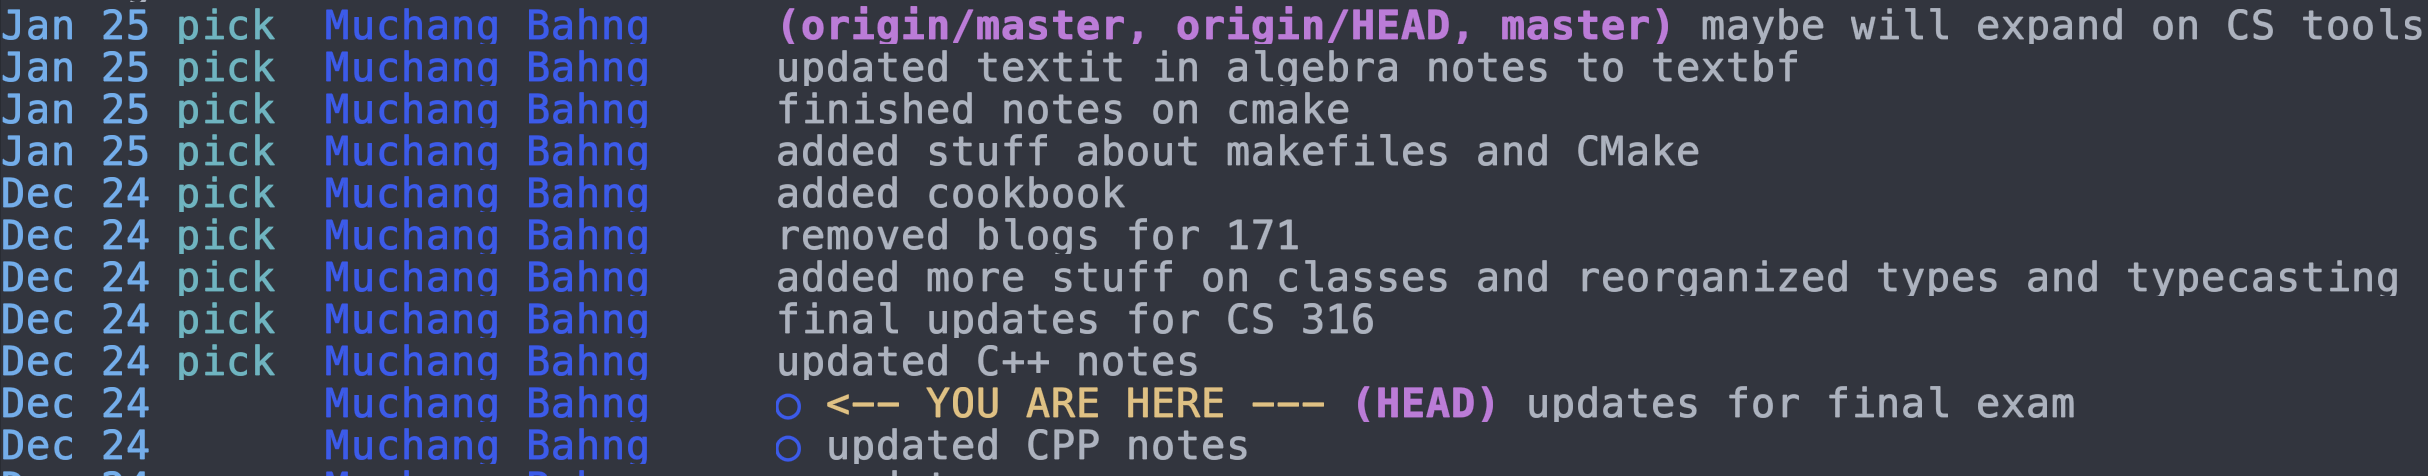
\includegraphics[scale=0.3]{img/rebase.png}
      \caption{Interactive rebase shown in LazyGit.} 
      \label{fig:rebase}
    \end{figure}

    There are a fixed set of supported operations allows in an interactive rebase.\footnote{Note that pick and reword will never cause conflicts. Squash and fixup will most likely not cause conflicts. Drop, break, edit, and swapping may cause conflicts.}
    \begin{enumerate}
      \item \textbf{Pick}. This just means that you are leaving the commit alone, i.e. picking it to be in the rebase. 
      \item \textbf{Reword}. Just edits the commit message. 
      \item \textbf{Squash}. Given commit $C_i \leftarrow C_{i+1}$, you can label $C_{i+1}$ with \texttt{squash} to merge it into $C_{i}$, turning 2 nodes into one. This almost never causes conflicts. The new commit message is just those of $C_{i}, C_{i+1}$ concatenated. 
      \item \textbf{Fixup}. Like squash, but discard the commit's message.  
      \item \textbf{Drop}. This deletes a commit and removes it entirely.  
      \item \textbf{Break}. Stop at this commit to edit it. I think you can change which edits you have committed, choose which edits to keep, and choose which edits to remove (back into your unstaged changes). 
      \item \textbf{Edit}. Stop at this commit to amend it. 
      \item You can also swap commits by editing the text file so that the commits are in a different order. 
        \begin{lstlisting}
          # Original order in rebase editor:
          pick abc123 First commit
          pick def456 Second commit

          # After swapping lines in editor:
          pick def456 Second commit
          pick abc123 First commit 
        \end{lstlisting}
    \end{enumerate} 
    After you edit the rebase text file and continue the rebase, git will do the following sequentially: 
    \begin{enumerate}
      \item \texttt{HEAD}, which pointed at $C_n$, will point towards $C_s$. 

      \item While \texttt{HEAD} is pointing at $C_i \neq C_n$ (i.e. not at the end), we do the following. 
        \begin{enumerate}
          \item It will attempt to perform all the operations you have specified for the next commit $C_{i+1}$. 
          \item If the operations are finished, we increment \texttt{HEAD} to point to $C_{i+1}$ and continue. 
          \item If there is a conflict, it will pause, state that there are conflicts between $\texttt{HEAD} = C_i$ and $C_{i+1}$, and ask you to resolve them. Once resolved it will continue. 
        \end{enumerate} 

      \item Then we are done with the rebase since we have went through all commits, modified them, and resolved all conflicts. 
    \end{enumerate}
    Interactive rebasing is an extremely powerful way to modify your commit history, and it's probably the operation where you'll spend the most time on git. 
  \end{definition} 

  Again, note that if you have changed anything in commit $C_i$, then the hash of $C_i$ every $C_j$ after will get changed. This causes git to interpret these changed commits as completely new ones, even if we only picked a given commit without any modifications. For single-branch rebases, this is fine, but this causes some nasty problems when rebasing over multiple branches, as we will talk about later. 

  \begin{definition}[Patching]
    An easier way to modify your edits in old commits is through \textbf{patching}.\footnote{Though patching really just does an interactive rebase in the backend.} Within a commit, a \textbf{patch} is simply a diff file that you can add and remove to. It's like having a mini-staging area in a commit. When you have selected the different files/lines you have added to your patch, you can either choose to: 
    \begin{enumerate}
      \item Remove them from the commit. 
      \item Add them to another commit. 
      \item Move them from the original commit to a new commit. 
    \end{enumerate}
  \end{definition}

  \begin{theorem}[Splitting Commits Into Two Different Commits]
    If you want to split commits, 
    \begin{enumerate}
      \item create a dummy commit 
      \item go to the commit you want to split, get its patches, and add them to the dummy commit. 
      \item Do an interactive rebase to swap the dummy commits down until you have it at the desired location. 
    \end{enumerate}
  \end{theorem} 

\subsection{Branches} 

    Okay, so we now have much better control over our git history, but we've only been treating our history as a linked list. In order to introduce the tree structure, we need to introduce the \textit{branch}. This is especially important if we have a particular previous commit $C_{k < n}$ where we would like to make some different changes to, giving us \textbf{diverging histories} with next nodes $C_k \leftarrow C_{k+1}$ and $C_k \leftarrow C_{k^\prime + 1}$. 
    
    \begin{definition}[Branch]
      A \textbf{branch} is a path from the root commit to any leaf node. It represents a unique history from genesis to \texttt{HEAD}. To list all branches, use 
      \begin{lstlisting}
        >> git branch 
          feature/threading
        * main
          test/tensor
      \end{lstlisting} 
      The asterisk represents which branch you are currently on. The first branch you start off with is a special branch called \textbf{main}, or \textbf{master} branch. 
    \end{definition} 

    Therefore, really our linked-list history is a git tree with a single branch. 

    \begin{definition}[Creating/Switching Branches]
      From any (main or non-main) branch you can create new branches by choosing the commit to split from. 
      \begin{enumerate}
        \item Create a new branch from HEAD of current branch. 
          \begin{lstlisting}
            git branch <new-branch-name> 
          \end{lstlisting}

        \item Create a new branch from certain commit of current branch. 
          \begin{lstlisting}
            git branch <new-branch-name> <commit-hash>
          \end{lstlisting} 

        \item To switch to another branch 
          \begin{lstlisting}
            git checkout <branch> 
          \end{lstlisting}
      \end{enumerate}
    \end{definition} 

  \subsubsection{Working Between Branches} 

    If you are simultaneously working on multiple branches, you may have to checkout/switch between branches frequently. Often, you may have uncommitted changes before you checkout, and git does not allow you to do this. Therefore, we can \textit{stash} them. 

    \begin{definition}[Stash]
      \textbf{Stashing} changes mean that you can take uncommitted changes and store them in a temporary node but not have it point to any existing commit in a branch. This allows you to save your changes without having to commit incomplete work to a branch, and you can pop them back whenever you need. 
    \end{definition} 

    Sometimes, you may want to just copy a commit from one branch to another. You can do this using an interactive rebase, but this may be overkill since it is mainly used to work with a sequence of commits. 

    \begin{definition}[Cherry-Picking and Pasting]
      You can do copy a commit by \textbf{cherry picking} it and \textbf{pasting} it somewhere else. 
    \end{definition} 

  \subsubsection{Integrating Branches} 

    The reason you want to have different branches is so that you have independent workflows that may hopefully be integrated into the master branch. So how does one actually perform this integration? There are two general ways to do this: a 3-way merge or a rebase. For both methods, we will use this example. 
    \begin{lstlisting}
      main     : A1 --- A2 --- A3
                                \
      feature1 :                 B1 --- B2 --- B3
                                \
      feature2 :                 C1 --- C2 --- C3
    \end{lstlisting}

    \begin{definition}[Fast-Forward Merge]
      If you want to merge \texttt{main} and \texttt{feature1}, notice that \texttt{feature1} is really just ahead of \texttt{main} by some number of commits. The easiest way to merge is to add the additional commits in \texttt{feature1} to \texttt{main}. This is called a \textbf{fast-forward merge}, which we can call using 
      \begin{lstlisting}
        git checkout main 
        git merge --ff-only feature1
      \end{lstlisting} 
      Doing so will result in 
      \begin{lstlisting}
        main     : A1 --- A2 --- A3 --- B1 --- B2 --- B3
                                  \
        feature1 :                  --- B1 --- B2 --- B3
                                  \
        feature2 :                  --- C1 --- C2 --- C3
      \end{lstlisting}
      and we can delete \texttt{feature1} since it's not needed. 
    \end{definition}

    In fact, if a fast-forward merge is possible, then calling \texttt{git merge feature1} will automatically do a fast-forward. We can explicitly set it to only attempt or never attempt fast-forward by adding the \texttt{--ff-only} or \texttt{--no-ff} flags. 

    \begin{definition}[3-Way Merge]
      If you want to merge two divergent branches, e.g. \texttt{feature1} and \texttt{feature2}, then a fast-forward is not possible. Rather, you want to choose to merge \texttt{feature2} \textit{into} \texttt{feature1}. Git will rather do a \textbf{three-way merge} between the divergent node \texttt{A3} and the heads of the respective branches \texttt{B3} and \texttt{C3}. After you resolve conflicts, the tree should look something like 
      \begin{lstlisting}
        main     : A1 --- A2 --- A3
                                  \
        feature1 :                  --- B1 --- B2 --- B3 --- M1
                                  \                          /
        feature2 :                  --- C1 --- C2 --- C3 ---
      \end{lstlisting}
      Note that we could choose to merge \texttt{feature1} into \texttt{main} subsequently, resulting in both feature branches merged. 
      \begin{lstlisting}
        main     : A1 --- A2 --- A3 ------------------------------- M2
                                  \                                 /
        feature1 :                  --- B1 --- B2 --- B3 --- M1 ---
                                  \                          /
        feature2 :                  --- C1 --- C2 --- C3 ---
      \end{lstlisting}
    \end{definition}

    Note that a three-way merge may result in a pretty ugly tree, especially if we are working with dozens of branches. What we would like to do is a three-way merge in a fashion that \textit{looks like} a fast-forward merge. That is, we want the main branch to have a linear structure rather than a series of diverging and converging nodes. In fact, we already have the tools to do this. Let's revisit the interactive rebase again. We have seen that we can do an interactive rebase from a start commit by doing 
    \begin{lstlisting}
      git rebase -i <start-commit-hash>
    \end{lstlisting} 
    What we would like to do is to rebase from a commit in a different branch. 

    \begin{definition}[Rebase]
      If we want to linearly merge \texttt{feature2} into \texttt{feature1}, this is called ``\textbf{rebasing} \texttt{feature2} \textit{onto} \texttt{feature1}.'' We run 
      \begin{lstlisting}
        git checkout feature2 
        git rebase feature1
      \end{lstlisting} 
      which means ``take my current branch's unique commits and replay them on top of whatever branch I am rebasing on (in here, \texttt{feature1}).'' This will result in 
      \begin{lstlisting}
        main     : A1 --- A2 --- A3
                                  \
        feature1 :                 B1 --- B2 --- B3
                                                  \
        feature2 :                                 C1' --- C2' --- C3' 
      \end{lstlisting} 
      where the \texttt{C'} are the same commits but with different hashes since they start from a different parent. 
    \end{definition} 

    \begin{example}[Updating Feature Branch with Changes from Main]
      A common workflow you would do in a large project with multiple developers is as follows. Consider that you are working on \texttt{feature1} and another developer is working on \texttt{feature2}. 
      \begin{lstlisting}
        main     : A1 --- A2 --- A3
                                  \
        feature1 :                  --- B1 --- B2 --- B3
                                  \
        feature2 :                  --- C1 --- C2 
      \end{lstlisting}
      Your friend pushes their changes to \texttt{main}, which leads to this structure. 
      \begin{lstlisting}
        main     : A1 --- A2 --- A3 --- C1 --- C2
                                  \
        feature1 :                  --- B1 --- B2 --- B3
                                  \
        feature2 :                  --- C1 --- C2 
      \end{lstlisting}
      Your branch has diverged from main, so you will need to rebase your own branch onto main. You checkout to \texttt{feature1} and run \texttt{git rebase main}. After settling conflicts, your branch will look like the following, updated with the most recent commits from \texttt{main}. 
      \begin{lstlisting}
        main     : A1 --- A2 --- A3 --- C1 --- C2
                                                \
        feature1 :                                --- B1' --- B2' --- B3'
                                  \
        feature2 :                  --- C1 --- C2 
      \end{lstlisting}
    \end{example}

    \begin{example}[Converting a Merge Into Rebase]
      Say that you already merged \texttt{feature1} and \texttt{main}. 
      \begin{lstlisting}
        main     : A1 --- A2 --- A3 ------------------------ M1
                                  \                          /
        feature1 :                  --- B1 --- B2 --- B3 ---  
      \end{lstlisting}
      You realized that you actually wanted to do a fast-forward so that it looks linear! How do you do this? 
      \begin{enumerate}
        \item You first undo the merge. 
          \begin{lstlisting}
            git checkout main 
            git reset --hard A3
          \end{lstlisting} 

        \item Then do the rebase of \texttt{feature1} onto \texttt{main}. 
          \begin{lstlisting}
            git checkout feature1 
            git rebase main 
          \end{lstlisting} 

        \item Then fast-forward to main to include \texttt{feature1}'s commits. 
          \begin{lstlisting}
            git checkout main 
            git merge --ff-only feature1
          \end{lstlisting}
      \end{enumerate}
      We will have this in the end. 
      \begin{lstlisting}
        main     : A1 --- A2 --- A3 --- B1' --- B2' --- B3' 
        feature1 : A1 --- A2 --- A3 --- B1' --- B2' --- B3'
      \end{lstlisting}
    \end{example} 

\subsection{Remote Trees}

  So far, we've talked about how you can use git to keep track of your edit history locally, but another benefit is to store these changes in the cloud. This is done through a third-party provider, and they are completely separate entities from git. The three most dominant ones are  
  \begin{enumerate}
    \item \textit{Github}. Owned by Microsoft and is the default for most open-source projects, with 100 million users. 
    \item \textit{Gitlab}. Owned by Gitlab and is slowly gaining popularity due to better control of repositories and after Microsoft acquired github. 
    \item \textit{Bitbucket}. Owned by Atlassian and used for private repositories in enterprise settings. 
  \end{enumerate}
  Again, all three platforms still use \textit{git}, but the cloud storage is managed separately. All of these platforms provide a remote server that stores all of these git histories of millions of repositories around the world. The motivation behind the need of a remote workspace is that it is a common ground in which many developers can communicate and track the progress of their entire repository. 

  \begin{definition}[Remote Repository]
    The first step to setting up a cloud-based git tree is to place it on some server (IP address) in some directory with the proper permissions. This remote location containing the git tree and the corresponding code is called the \textbf{remote repository}, and it is encoded in either a URL or a SSH host link of the form 
    \begin{lstlisting}
      https://github.com/user/repo.git
    \end{lstlisting} 
    For now, we will consider a local repository having at most 1 remote repository that it can communicate to.\footnote{When we get to forking, we will talk about multiple remote repositories.} Conventionally, the primary\footnote{Again, for now it's really the only remote.} remote repository goes under the alias \textbf{origin}. 
  \end{definition}  

  None of the commands that we have introduced so far does anything to the remote repository. The first command we should know is how to set up one from scratch. 

  \begin{definition}[Add Remote]
    Given that git is initialized, we can initialize a corresponding remote repository by running 
    \begin{lstlisting}
      git remote add <remote-name> <remote-url>
    \end{lstlisting}
    Again, conventionally the \texttt{<remote-name>} is put as \texttt{origin}. 
  \end{definition} 

  Great, we have set a remote repository up, but there is an extra step to do. Most synchronizations happens at a branch level rather than the whole tree itself, so what we would need to do for each local branch is create a corresponding remote branch and then \textit{connect} those two so that git knows which branches to sync together. The local branch is called the \textbf{downstream} branch and its corresponding remote branch is called \textbf{upstream}. 

  In order to understand how the process of setting upstream branches is done, we introduce another variable in our local repository. In our local git tree, we have stated that for each branch \texttt{B}, there is a \texttt{HEAD} pointer living at the most recent commit, denoted as \texttt{B/HEAD} or just \texttt{B}. 

  \begin{definition}[Remote References] 
    There is actually a second pointer called the \textbf{remote reference (ref)} in the local branch called \texttt{origin/B} (more generally \texttt{<remote>/<branch>}), which is a symbolic link that points to the head of the remote branch. They are git's way of keeping track of the state of branches in your remote repositories. 
  \end{definition} 

  For some local branch, the existence of a remote ref tells you where the corresponding upstream branch is located (i.e. at \texttt{<remote>/<branch>}). If you do not see the remote ref, this means that you have not yet connected your local branch to its remote upstream, which can happen if the remote counterpart doesn't exist (i.e. you created a completely new branch) or you have never connected it. You can find all local branches and the remote references by calling 
  \begin{lstlisting}
    git branch -vv
    # Shows all branches with their tracking info
    # Example output:
    # * main    abc123 [origin/main] Latest commit message
    #   feature def456 [origin/feature: ahead 2] Some work
  \end{lstlisting} 

  \begin{definition}[Push with Set Upstream] 
    We consider two cases, where we do not see the remote refs at all. 
    \begin{enumerate}
      \item Say that you have a local branch \texttt{main} with some committed changes, and the remote branch does not exist at all. Your tree will look something like this 
        \begin{lstlisting}
          Remote: 
          Local : A <- B <- C <- (main) D
        \end{lstlisting}
      \item Say that you have a local branch \texttt{main} with some committed changes, and the remote branch does exist but the upstream is not set. 
        \begin{lstlisting}
          Remote: A <- (main) B
          Local : A <- B <- C <- (main) D
        \end{lstlisting}
    \end{enumerate}
    We can synchronize our local commits with the remote repo by \textbf{pushing} them. As we push, we also set the upstream with the \texttt{-u} or \texttt{--set-upstream} flag. 
    \begin{lstlisting}
      git push -u <remote> <branch> 
      
      # for example, if we want to push our current checked out branch to origin/main
      git push -u origin main
    \end{lstlisting}
    This will set your remote refs, and in both cases we will have 
    \begin{lstlisting}
      Remote: A <- B <- C <- (main) D
      Local : A <- B <- C <- (main, origin/main) D
    \end{lstlisting}
  \end{definition}

  \begin{definition}[Push] 
    If your remote ref is already set and you have some further commits, 
    \begin{lstlisting}
      Remote: A <- B <- C <- (main) D
      Local : A <- B <- C <- (origin/main) D <- E <- (main) F
    \end{lstlisting}
    then you can just push your changes with \texttt{git push}, which will push the commits up to HEAD and update the remote ref to HEAD. 
    \begin{lstlisting}
      Remote: A <- B <- C <- D <- E <- (main) F
      Local : A <- B <- C <- D <- E <- (main, origin/main) F
    \end{lstlisting}
  \end{definition} 

  In all of these scenarios, we have only seen cases when \texttt{origin/main} and \texttt{main} point to the same commit. However, remember that the remote ref is a \textit{local} pointer to the remote repo's head, and so it is only updated every time your local repo interacts with the remote repo. Therefore, they can be different. 

  \begin{example}[Remote Ref is Different From True Remote Head]
    Say that you are \texttt{Local1} and a friend is \texttt{Local2}. We first start off with this. 
    \begin{lstlisting}
      True Remote: A <- B <- C <- (main) D
      Remote1    : A <- B <- C <- (main) D 
      Local1     : A <- B <- C <- (main, origin/main) D 
      Remote2    : A <- B <- C <- (main) D
      Local2     : A <- B <- C <- (main, origin/main) D
    \end{lstlisting}
    Your friend makes commits \texttt{E} and \texttt{F} and pushes them while you are working on commit \texttt{G}.  
    \begin{lstlisting}
      True Remote: A <- B <- C <- D <- E <- (main) F
      Remote1    : A <- B <- C <- (main) D 
      Local1     : A <- B <- C <- (origin/main) D <- (main) G
      Remote2    : A <- B <- C <- D <- E <- (main, origin/main) F 
      Local2     : A <- B <- C <- D <- E <- (main, origin/main) F 
    \end{lstlisting} 
    In this case, your friend's push will update the head of the remote main branch to \texttt{F} and update their remote ref to \texttt{F} as well. But you have worked only locally and have no interacted with the remote repo for a while, so your remote ref is still \texttt{D}. When you therefore try to push your changes, git will complain to you that your future ref and the remote head does not match. Since this creates divergent histories which splits from \texttt{D}, it will not let you push. 
  \end{example}

  The scenario above is clearly a problem, and it stems from the fact that we have a remote ref. Why need remote refs at all if they seem redundant and at the same time they might introduce this problem? The answer is convenience. Imagine that there were no remote refs. This means that every time someone pushed to the remote main I would need to be notified that there were changes to main. However, I may not have access to the remote repo while I am working on my code, so I may still have the same problem when I am able to connect. The extra remote ref pointer allows for quick checking to see if my local branch matches its upstream. It turns out that if the upstream changed, git does indeed warn you about it as soon as possible. 

  \begin{definition}[Fetch] 
    Say that for a branch, it looks like this, and your local remote is not updated with the true remote's latest commits. 
    \begin{lstlisting}
      True Remote: A <- B <- C <- D <- E <- (main) F
      Remote1    : A <- B <- C <- (main) D 
      Local1     : A <- B <- C <- (origin/main, main) D
    \end{lstlisting}
    To update your remote ref to match the current upstream head, we can \textbf{fetch} it to get the following. 
    \begin{lstlisting}
      True Remote: A <- B <- C <- D <- E <- (main) F
      Remote1    : A <- B <- C <- D <- E <- (main) F
      Local1     : A <- B <- C <- (main) D <- E <- (origin/main) F
    \end{lstlisting}
    It comes in three commands. 
    \begin{lstlisting}
      git fetch <remote-url> <branch> # fetches from specific remote branch 
      git fetch <remote-url>          # fetches from all branches in a remote repo  
      git fetch                       # fetches from all branches of all remote repos
    \end{lstlisting}
  \end{definition}

  \begin{definition}[Fast-Forward]
    In the case above, note that even though the commits are synchronized to your local remote, the changes aren't actually reflected in your current code since HEAD has not moved. If you want head to also move to the most recent remote ref, then you can do a \textbf{fast-forward merge}. 
    \begin{lstlisting}
      True Remote: A <- B <- C <- D <- E <- (main) F
      Remote1    : A <- B <- C <- D <- E <- (main) F
      Local1     : A <- B <- C <- D <- E <- (origin/main, main) F
    \end{lstlisting}
    You can do this in git by checking out to the local branch you are on. After fetching, you should have the remote ref that you want to update your HEAD to, which you put in as an argument. 
    \begin{lstlisting}
      git merge --ff-only <remote-url/branch> 
      # e.g. 
      git merge -ff-only origin/main 
    \end{lstlisting}
  \end{definition}

  \begin{definition}[Pull]
    The combination of doing a fetch to get the latest commits and update the remote ref, and then doing a (fast-forward) merge to update your HEAD pointer to the remote ref, is so common that we refer to doing these two things sequentially as a \textbf{pull}. Therefore, the two commands are the same. 

    \noindent\begin{minipage}{.5\textwidth}
      \begin{lstlisting}[]{Code}
        git pull <remote-url> <branch> 

        git fetch <remote-url> <branch>  
        git merge <remote-url/branch>
      \end{lstlisting}
      \end{minipage}
      \hfill
      \begin{minipage}{.49\textwidth}
      \begin{lstlisting}[]{Output}
        git pull origin main 

        git fetch origin main 
        git merge origin/main
      \end{lstlisting}
    \end{minipage}
  \end{definition}

  \begin{definition}[Clone]
    Finally, you can take an existing remote repository and \textbf{clone} it, which creates a complete copy of a remote repository. It does the following. 
    \begin{enumerate}
      \item Does a \texttt{git init} to set up git. 
      \item Does \texttt{git remote add origin <remote-url>} to connect to the remote repo and set the \texttt{origin} alias to it. 
      \item Does \texttt{git fetch origin} to fetch all branches of the remote repo, setting up the local remote branches and their corresponding remote refs. 
      \item Does \texttt{git checkout -b main origin/main} which creates the local branch \textbf{main}, checks out to it, and sets \texttt{origin/main} as its upstream. 
    \end{enumerate}
  \end{definition}

\subsection{Reflog} 

  \begin{definition}[Reflog]
    Git's \textbf{reflog} is a super-history that records every change to your branch tips. It's essentially an undo tree for all git actions (sort of like a meta undo tree). Therefore, if you ever screwed something up, git allows you to undo your actions by undoing the entries in the reflog. It contains the following types of actions. 
    \begin{enumerate}
      \item Branch Operations
        \begin{itemize}
          \item checkout: switching branches
          \item branch: creating/deleting branches
          \item merge: merging branches
          \item rebase: rebasing branches
          \item pull: pulling from remote
        \end{itemize}
      
      \item Commit Modifications
        \begin{itemize}
          \item commit: new commits
          \item reset: moving HEAD
          \item revert: reverting commits
          \item amend: amending commits
          \item cherry-pick: copying commits
        \end{itemize}

      \item Stash Operations
        \begin{itemize}
          \item stash: stashing changes
          \item stash apply: applying stash
          \item stash pop: popping stash
        \end{itemize}

      \item History Rewrites
        \begin{itemize}
          \item rebase -i: interactive rebase
          \item filter-branch: rewriting history
        \end{itemize}

      \item Reference Updates
        \begin{itemize}
          \item HEAD@{n}: moving HEAD pointer
          \item refs/heads/*: branch pointer updates
          \item refs/remotes/*: remote branch updates
          \item refs/stash: stash reference updates
        \end{itemize}

      \item Remote Operations
        \begin{itemize}
          \item clone: cloning repository
          \item fetch: fetching from remote
          \item push: pushing to remote
          \item remote add: adding remote
        \end{itemize}
    \end{enumerate}
    You can access it using the following command. 
    \begin{lstlisting}
      $ git reflog
      ab12345 HEAD@{0}: reset: moving to HEAD~1    # Most recent action
      bc23456 HEAD@{1}: commit: Add feature X 
      cd34567 HEAD@{2}: rebase: onto main          # Rebase happened here
      ef45678 HEAD@{3}: commit: Initial commit
    \end{lstlisting}
  \end{definition}

\subsection{Pull Requests and Forking} 

